
\chapter[Sub Energia]{Sub Energia}

\section{Objetivo Específico}

Dimensionar o sistema de arrefecimento e de admissão de um motor a combustão interna e de um dinamômetro de bancada. Com isso analisar as transferências de calor presentes no sistema, o fluxo de ar, consumo de combustível, desempenho do motor e emissões gasosas.

Fazer a instalação elétrica do dinamômetro de bancada juntamente com seu ligamento a rede.

\section{Recursos}

Para estudo de emissões gasosas será utilizado um analisador de gases (PC-Multigás NAPRO) como CO, CO$_{2}$, HC, O$_{2}$, NO$_{x}$. Esse equipamento será conectado ao sistema de exaustão obtendo dados por meio do método de medição de infravermelho não dispersivo. 

O processo de instalação elétrica do dinamômetro será auxiliada por um técnico especializado por questão de segurança, já que se trata de um sistema de alta tensão. Os equipamentos de proteção individual (EPIs) utilizados pertencem a Faculdade Gama UnB.

\section{Concepção e detalhamento do subsistema}

\subsection{Sistema de Arrefecimento}

Em motores automotivos o arrefecimento é geralmente feito à líquido. Este líquido é um fluido refrigerante que, sendo bombeado por entre as camisas do motor e pelo cabeçote, resfria os componentes e, em seguida, passa pelo radiador onde ocorrerá a transferência de calor no sentido de dissipar o calor absorvido \cite{energiaToyota}.

O sistema de arrefecimento deve ser dimensionado para as condições em que estará submetido, não podendo estar subdimensionado para que não haja um superaquecimento do motor. É composto por uma bomba, uma válvula termostática, um radiador e um fluido refrigerante. A bomba d'água é acionada pela correia de sincronismo o que garante que a rotação da bomba e sua vazão sejam proporcionais a rotação do motor \cite{energiaToyota}. 

A válvula termostática é feita por uma cera derivada do petróleo que se expande ao ser aquecida, forçando a abertura para a saída do líquido de arrefecimento quando o motor já estiver aquecido, ao mesmo tempo que impede que ele esfrie em condições de baixa temperatura externa \cite{energiaToyota}.  

O fluido refrigerante é composto por uma solução de água e etilenoglicol. O etilenoglicol em solução com a água permite que, em determinadas concentrações, a solução possua um ponto de congelamento a temperaturas inferiores a 0$^{\circ}$C e um ponto de ebulição a temperaturas superiores a 100$^{\circ}$C \cite{energiaToyota}. %adicionar Graus

O radiador é uma superfície aletada onde ocorrem as trocas de calor com o ambiente. As aletas são utilizadas para aumentar a transferência de calor com o ambiente e aumentam muito a taxa de transferência de calor com a partir da superfície.  Esse efeito ocorre devido às várias folhas finas de metal que são colocadas nos tubos de água quente e que aumentam várias vezes a superfície de convecção \cite{energiaTransferencia}.

Todo o sistema de arrefecimento já está presente no motor que será utilizado para os testes . Serão colocados dois sensores de temperatura antes e depois do radiador para que possam ser efetuados os cálculos da transferência de calor, bem como monitorar a temperatura do líquido de arrefecimento. Conhecendo-se a temperatura do fluido na entrada e a temperatura na saída, a taxa de transferência de calor a partir do fluido de resfriamento para o ar é dada por:

\begin{equation}
	Q = mc_{p}t = mc_{p}(T_{e} - T_{s})
\end{equation}

Para determinar a efetividade do trocador de calor será dada por:

\begin{equation}
	\varepsilon = \frac{Q}{Q_{max}}
\end{equation}

$Q_{max}$ é a taxa de transferência de calor máxima possível dada por:

\begin{equation}
	Q_{max} = c_{min} \times (T_{1} - T_{2})
\end{equation}

$C_{min}$ é a menor capacidade térmica entre os fluidos do trocador

\begin{equation}
	C_{min} = m \times c_{p}
\end{equation}

$T_{1}$: Temperatura de entrada do fluido de maior capacidade térmica

$T_{2}$: Temperatura de entrada do fluido de menor capacidade térmica

$m$ : Vazão mássica do fluido (kg/s)

$c_{p}$ : Calor específico a pressão constante (J/kg.K)

\subsection{Sistema de Admissão}

O Sistema de Controle de Admissão de Ar  - SCAA do projeto tem o objetivo de avaliar o fluxo de ar (volume por unidade de tempo) que é admitido para o interior da câmara de combustão do motor. 

As informações do SCAA e do Sistema de Controle de Escape de Gases - SCEG permite identificar, através de testes, a composição ideal em porcentagem da mistura ar/combustível para atingir o melhor consumo de combustível (combustão completa). 

O SCAA será fixado no coletor de ar do motor em análise pela Bancada de Teste de Motores - BTM. O SCAA é composto por uma luva metálica, tubulação metálica, um fluxômetro, e uma válvula de controle de entrada de ar. A luva metálica acoplará o coletor de ar do motor à tubulação metálica onde serão fixados o fluxômetro e válvula de controle de entrada de ar. As informações do fluxo serão enviadas para a Central de Controle de Dados - CCD. A válvula de controle de entrada de ar será ajustada via computador.

\subsection{Instalação do Dinamômetro}

Para funcionamento deste equipamento, será necessário um amplo estudo de viabilidade técnica e financeira. A unidade de controle do dinamômetro funciona em alta voltagem, por isso necessita de um projeto de sistema de aterramento para segurança, dimensionamento do cabeamento.

O projeto de aterramento se resume nas seguintes etapas:

\begin{enumerate}
	\item Entrada dos dados básicos de projeto
	\begin{itemize}
		\item Modelagem do solo;
		\item Determinação da corrente de falta máxima que fluirá pelo aterramento;
		\item Área a ser utilizada para instalação do aterramento; 
	\end{itemize}
	\item Determinação da corrente máxima tolerável pelo corpo humano e das tensões de passo e de toque admissíveis
	\item Proposta de arranjo inicial dos eletrodos
	\item Avaliação da resistência de aterramento, da distribuição de potenciais no solo, e da elevação de potencial da malha
	\item Revisão e refinamento da malha de aterramento
\end{enumerate}

A partir de uma análise da demanda de energia elétrica na Faculdade Gama durante vários momentos do dia, será escolhido o horário em que a demanda for menor para realização dos testes de acordo com o gráfico gerado (energia elétrica consumida x tempo).

\subsection{Análise de teste}

Posteriormente a finalização do projeto, serão realizados testes que demonstram a sua funcionalidade de forma que sirva como material didática para possíveis estudos. Dentres eles, será analisado o consumo de combustível e emissões gasosas com diferentes misturas de combustíveis. 

A medição do consumo de combustível será analisada pelo método volumétrico. Para isso, utiliza-se uma bureta graduada como da figura \ref{buretaGraduada} na linha de alimentação e por meio da diferença no nível de combustível para um determinado intervalo de tempo de funcionamento do motor será fornecido o volume consumido.

\begin{figure}[h!]
	\centering
	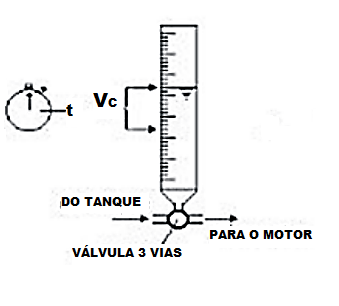
\includegraphics[keepaspectratio=true,scale= 0.7]{figuras/bureta-graduada.PNG}
	\caption{Bureta para medida volumétrica do consumo de combustível}
	\label{buretaGraduada}
\end{figure}

A maior fonte de poluição urbana do ar pode ser relacionado com o motor a combustão interna ciclo Otto e ciclo Diesel (HEYWOOD, 1988). Além do gás carbônico produzido nas reações de combustão, outros gases também são formados, como  o monóxido de carbono (CO), óxidos de nitrogênio (NOx), hidrocarbonetos (HC), oxigênio (O2), compostos orgânicos voláteis (COVs), entres outros.

Ao conhecer os mecanismos de formação de poluentes gerados pelo motor, pode-se associar a tecnologias de gerenciamento de controle. Com isso, compreende-se que os níveis de emissões gasosas veiculares podem ser controlados e regulamentados, adequando-se aos padrões exigidos pela legislação e buscando uma menor poluição do meio ambiente. 

O órgão que delimita os limites legais de emissões veiculares, no Brasil, é o Conselho Nacional do Meio Ambiente (CONAMA). Para a implementação das resoluções, citadas na Tabela 1, o CONAMA criou o Programa de Controle da Poluição do Ar por Veículos Automotores (PROCONVE) para os veículos leves e pesados, fixando prazos, limites máximos de emissões e estabelecendo exigências tecnológicas para veículos automotores, nacionais e importados \cite{energiaAvaliacao}.

\begin{table}[h!]
	\centering
	\caption{Resoluções CONAMA aplicadas a veículos no Brasil \cite{energiaAvaliacao}.}
	\label{resoluçõesConama}
	\begin{tabular}{|l|l|l|l|}
		\hline
		\multicolumn{4}{|c|}{RESOLUÇÕES CONAMA} \\ \hline
		Nº 01/1993      & Nº 07/1993;      & Nº 226/1997     & Nº 297/2002;     \\ \hline
		Nº 08/1993      & Nº 14/1995;      & Nº 242/1998;     & Nº 315/2002;     \\ \hline
		Nº 15/1995      & Nº 16/1995      & Nº 282/2001;     & Nº 415/2009.     \\ \hline
	\end{tabular}
\end{table}

\section{Levantamento de Custos}

Sistema de Arrefecimento: para análise da transferência de calor no sistema de arrefecimento serão utilizados os equipamentos já existentes do motor utilizado, além dos sensores que foram incluídos nos custos do subsistema de eletrônica. Portanto, não haverão custos extras neste subsistema. 

A tabela a seguir estima aproximadamente os valores gastos para o desenvolvimento de estudo do subsistema de energia.

\begin{table}[h!]
	\centering
	\caption{Detalhamento dos recursos e custos associados no subsistema.}
	\label{detalhamentoRecursos}
	\begin{tabular}{|l|l|l|}
		\hline
		\multicolumn{1}{|c|}{}   & \multicolumn{1}{c|}{Descrição} & \multicolumn{1}{c|}{Valor} \\ \hline
		Sistema de arrefecimento &                                &                            \\ \hline
		Sistema de admissão      &                                &                            \\ \hline
		Análise de emissões      & Analisador de gases compacto   & R\$ 8000,00                 \\ \hline
		Consumo de combustível   & Bureta graduada                & R\$ 70,00                   \\ \hline
	\end{tabular}
\end{table}

